
Three findings in the eighteenth century led scientists to conclude that the brain used nerves as "wires": Benjamin Franklin and his many electrical discoveries (conservation of change, positive and negative charges, etc.), Luigi Galvani and his elecro-muscular experiments, and Emil du Bois-Reymond's discovery that the brain generates electricity. At this time there was much debate as to whether or not nervous signals were bidirectional; that is, if a single nervous chain sent signals to the brain for senses and similtanously sent signals from the brain for movement.

\begin{figure}[H]
  \begin{center}
    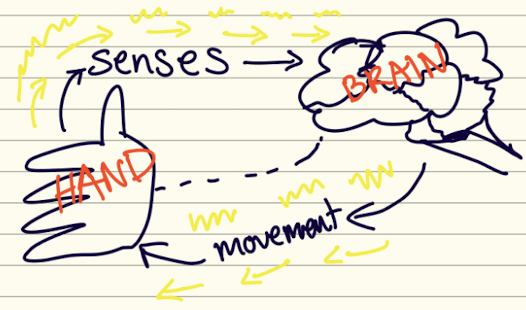
\includegraphics[width=0.65\textwidth]{figures/bidirectional}
  \end{center}
  \caption{}\label{fig:}
\end{figure}

In the early nineteenth century Charles Bell and Fran\c{c}oise Magendie ended the bidirectional controversy: they discovered that at the base of the spinal cord, just before the nerves attached, the nervous fibers divide into two brances/ roots: the dosal and ventral roots; the former responsible for sensorial information (coming in) and the latter responsible for muscular-electrical motor control (going out). This meant the nervous system was unidirectional. Bell conjectured that motor fibers come out from the cerebellum and that dorsal fibers terminate at the cerebrum. However, like Galen, he lacked any formal scientific evidence. Later, the physiologist Marie-Jean-Pierre Flourens rectified this. Through expiriments on birds, via severing strategic brain portions, he determined that this was indeed true. It is important to mention here that Flourens also performed these experiments on dogs and puppies, which recived criticism from his contemporary, Bell. 

\begin{figure}[H]
  \begin{center}
    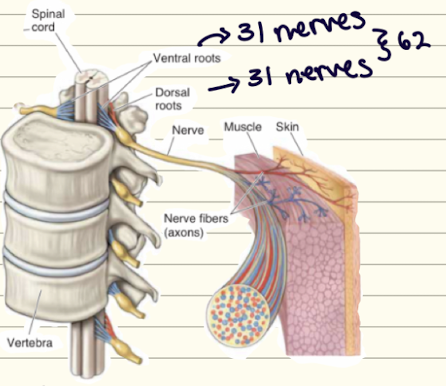
\includegraphics[width=0.30\textwidth]{figures/nervesplit}
  \end{center}
  \caption{}\label{fig:}
\end{figure}




